\documentclass[titlepage]{article}

\usepackage{amsmath}
\usepackage{amsfonts}
\usepackage{graphicx,picture,calc}
\usepackage{tikz}
\usepackage{url}
\usepackage{subfig}
\linespread{2}
\usepackage{float}

\usepackage{epsfig}

\usepackage{lineno}
\linenumbers

\usepackage[affil-it]{authblk}

\usepackage{natbib}
\bibliographystyle{mee}
\bibpunct{(}{)}{;}{a}{}{;}

%opening
\title{Using balanced acceptance sampling as a master sample for environmental surveys}
%\author{Paul van Dam-Bates, Oliver Gansell, \& Blair Robertson}

\author[1,*]{Paul van Dam-Bates}
\author[2]{Oliver Gansell}
\author[3]{Blair Robertson}

\affil[1]{%
	Department of Conservation, Christchurch, New Zealand 
}
\affil[2]{%
	Department of Conservation, Hamilton, New Zealand}

\affil[3]{%
	University of Canterbury, Christchurch, New Zealand}

\affil[*]{Corresponding author: Paul van Dam-Bates, pbates@doc.govt.nz}


\begin{document}

\maketitle


\begin{abstract}
Well designed environmental monitoring programmes for management organisations are important for evidence based decision making. However, many environmental problems are not single agency, single spatial scale issues. A master sample can be used to coordinate and scale monitoring designs to ensure consistency in information gathered and robustness of estimators at the different spatial scales. We propose using balanced acceptance sampling (BAS) to generate a master sample. Using Bas as a master sample is flexible, effective and improves on other methods previously explored. Some practical aspects of the design are addressed such as inclusion of legacy monitoring programmes, stratification, unequal probability sampling, rotating panel designs, and regional intensification. We explore the impact of including legacy monitoring through a simulation study. An example master sample is presented for environmental monitoring in New Zealand.

\end{abstract}

{\bf Keywords:} Master Sample, Spatial Balance, Environmental Monitoring, Legacy Monitoring.

\section{Introduction}

Environmental management agencies rely on the results of monitoring to answer questions about the success of their policies and programmes. Monitoring is often designed to address informations needs for a particular site or small set of sites. The quality of monitoring designed for site specific needs can vary greatly. Poor monitoring design can result in failure to provide meaningful data to inform management and policy decision making \citep{Legg2006, Nichols2006, Field2007}. Extrapolating from these studies to answer larger scale questions can introduce bias into the estimates as single sites are rarely representative of a broader region \citep{Peterson1999, dixon1998measuring}. 

Increasingly there is a need to monitor natural resources across broad spatial scales (ref). This is often undertaken by different agencies, which may or may not share the same purpose or objectives. This can to divergent approaches to monitoring even though the resource of interest is the same \citep{LarsenOlsenStevens2008}. Coordinating monitoring requires consistent approaches to the formulation of goals and objectives, selection of indicators and measures, field protocols and sample design \citep{fancy2009monitoring, LarsenOlsenStevens2008}. Material exists to assist in creating a well designed monitoring programme \citep{Gitzen2012, Reynolds2016, Vos2000} but coordination is required to ensure it is carried out properly and that standards are consistently applied. If one agency establishes monitoring locations using standard methods and sample design, another agency can use that data for their own purposes, reducing the need to establish more monitoring. By agencies working together and through a well set out design process the chances of monitoring being successful are higher. Concerns about the extrapolating estimates from disparate data sources is also reduced.

One way to coordinate sample design is to develop a master sample; a set of points that can be sub-sampled for different monitoring activities. This was first proposed by \citep{King1945}, but only recently has been introduced to environmental monitoring \citep{LarsenOlsenStevens2008, theobald2016} with implementation in the Pacific Northwest of the United States. Having different studies draw samples from the master sample has the benefit of enhancing collaboration within and between agencies to reduce duplication of effort. Additionally, consistent sample design has benefits when making estimates using data from multiple sources. Similar to providing standard field methods, the master sample provides standardised locations for sampling that ensures objective, unbiased estimation of the population parameters of interest. This coordination reduces convenience or judgement sampling and requires the user to define the objectives and sample frame clearly before gaining access to the sampling locations. 

The sampling method chosen should be flexible enough for a variety of users and study designs to be effective for coordination. Monitoring can take place on different spatial scales such as a national monitoring programme or a local one, investigating the impact of management action. When designing an individual study, identifying heterogeneity and using stratification \citep{Yoccoz2001} or unequal probability sampling \citep{Stevens1997} can produce more precise estimates. The study may need a unique balance of status and trend estimation which can be done by defining panels that have different revisit schema \citep{Skalski1990, Mcdonald2003, StevensOlsen1999}. In all these cases the sub-samples used must unbiased and representative.

The New Zealand Department of Conservation (DOC) is the lead biodiversity management agency in New Zealand. It is progressively implementing a coordinated monitoring and reporting system. Existing legacy monitoring include a national sample of Public Conservation Land (PCL) and various projects established to address specific local issues with diverse sample designs and methods employed. Development of the monitoring system has exposed the challenges in coordinating monitoring design to provide results meaningful at a local, regional and national scales. Increasingly partner environmental agencies (local government etc.) and central government expect cross-agency collaboration and coordination of systems and processes. Considerable effort has gone into a coordinated approach to selection of indicators and measures and field protocols \cite{DOC}. A master sample is one tool to have a coordinated approach to generation of sample designs.  

There are many ways to generate effective samples which could be used to coordinate monitoring. A simple random sample is unbiased but is less efficient than spatially balanced designs in the presence of spatial autocorrelation \citep{Grafstrom2013}. A design is spatially balanced if the sample is well-spread over the population --- a sample with few clumps and voids. A systematic sample can be considered near perfect spatial balance but is less flexible to changes in sample size making it a poor choice. Spatially balanced sampling designs are commonly used for sampling natural resources and a variety of designs have been proposed. \cite{StevensOlsen2004} introduced Generalized Random Tessellation Stratified (GRTS) design, a spatially balanced design that is frequently used in environmental monitoring. GRTS hierarchically orders a population using a base four numbering scheme and then selects a systematic sample from the ordered population. Another spatially balanced design is the Local Pivotal Method (LPM) \citep{Grafstrom2012}. LPM iteratively updates each sampling unit's inclusion probability in a way that makes it very unlikely to include neighbouring units in a sample. Once $n$ units have an inclusion probability of one, the sample is released. Although the spatial balance of LPM is better than GRTS, it is computationally prohibitive on large populations. For large populations, \cite{Grafstrom2014} introduced a new rapid implementation of LPM, called suboptimal LPM. LPM has better spatial balance, but suboptimal LPM is computationally feasible on large populations.

GRTS has been used to generate environmental monitoring master samples \citep{LarsenOlsenStevens2008}. The design is particularly useful for generating master samples because GRTS points are ordered using a reverse hierarchical ordering strategy that ensures that all contiguous sub-samples are also spatially balanced \citep{StevensOlsen2004}. By taking a large GRTS oversample, an ordered master sample can be obtained from which spatially balanced sub-samples can be drawn. However, once an oversample is chosen, it is not possible to generate additional points and this needs to be accounted for at the planning stage. \citet{theobald2016} also uses an adaptation of GRTS, Reversed Randomized Quadrant-Recursive
Raster (RRQRR), implemented in ArcGIS software \citep{theobald2007} to coordinate monitoring effort. The authors' are not aware of an ordering strategy for the LPM methods and hence, it is not clear how these methods could be used for oversampling. Another spatially balanced design is balanced acceptance sampling (BAS) \citep{Robertson2013}. It uses a quasi-random number sequence to generate spatially balanced points. Similar to GRTS, the outcome of the sequence is an ordered set of points such that any contiguous sub-sample maintains spatial balance. To generate a master sample with BAS, a random-start is chosen and after that an infinite set of points exist for the sample. Hence, the oversample size does not need to be specified for BAS.

This paper describes the development of a master sample for environmental monitoring in New Zealand, with a focus on terrestrial sampling of an area frame in which all sub-samples have positive area. We investigate using BAS to generate a master sample; how the points will be generated and then used in a for a range of applications. These include adapting to different spatial scales, stratification and unequal probability sampling, changes in boundaries or resources, revisitation structure (panel design), and inclusion of legacy monitoring. We will then provide an example for how this could be applied at the regional and national level in New Zealand.

\section{Methods}
\subsection{Point selection}

Two-dimensional BAS points are drawn from a random-start Halton sequence $\{{\bf x}_k\}_{k=1}^{\infty} \subset [0,1)^2$. The $i$th coordinate of each point in the sequence has an associated base $b_i$, with $b_1 = 2$ and $b_2 = 3$. The $i$th coordinate of the $k$th point in this sequence is (Robertson et al.\ 2017)
$$
x_k^{(i)} = \sum_{j = 0}^{\infty} \left\{\left\lfloor \frac{u_i + k}{b_i^j} \right\rfloor \text{ mod } b_i \right\}\frac{1}{b_i^{j+1}},
$$
where $u_i$ is a random non-negative integer and $\lfloor x \rfloor$ is the floor function --- the largest integer that is less than or equal to $x$. The two-dimensional random-start Halton sequence is 
\begin{equation}\label{BASeq}
\{{\bf x}_k\}_{k=1}^{\infty} = \left\{x_k^{(1)}, x_k^{(2)}\right\}_{k=1}^{\infty}.
\end{equation}

Setting $u_1 = u_2 = 0$ gives the classical Halton sequence \citep{Halton1960}. The points from eqn (\ref{BASeq}) are scaled to a minimal bounding box enclosing the study area and the first $n$ scaled points in the study area define the BAS sample. The BAS points are kept in the same order as they appear in eqn (\ref{BASeq}) and will have good spatial spread over the study area. Furthermore, any continuous subset of the BAS sample will also have good spatial spread \citep{Robertson2017}. Figure \ref{grid} shows an example of how this sequence creates spread by systematically choosing between boxes generated by the choice of the co-prime bases.

The random integer vector in the sequence ${\bf u} = (u_1, u_2) \in [0,10^7]^2$ is chosen so that ${\bf x}_1$ falls within the sample area \citep{Robertson2017}. This gives $O(\lambda 10^{14})$ possible BAS samples of size $n$, where $\lambda$ is the fraction of the bounding box occupied by the study area. By ensuring the random start comes from a large set of integers, the BAS points are uniformly distributed \citep{Robertson2013}. Once the random-start is selected an infinite number of BAS points exist over the study which constitutes the master sample. Higher dimensional points can be defined by using different co-prime bases for each additional dimension (e.g. $b_3 = 5$ when sampling from a $[0,1)^3$).

\subsection{Spatial Scales}
The Master sample should work at different spatial scales to answer national, regional, and local objectives. Let $A$ be a measurable subset of the study area for which the master sample is defined. Because the master sample $\{{\bf x}_k\}_{k=1}^{\infty}$ is uniformly distributed over $[0,1)^2$ \citep{Wang2000}, there exists a subsequence $\{{\bf z}_j\}_{j=1}^{\infty} \subset \{{\bf x}_k\}_{k=1}^{\infty}$ such that each ${\bf z}_j \in A$. Furthermore, $\{{\bf z}_j\}_{j=1}^n$ is a BAS sample of size $n$ drawn from $A$, with its random start and bounding box defined by the master sample. Hence, BAS samples can be drawn from the master sample at any spatial scale within the study area of the master sample.

What this means is that a national sample can share locations with monitoring at the local level. Let's say that nationally 1000 sites are generated, each with a unique order. If a sample of a region is taken and by chance 10 of these sites are shared, then the first ten sites in the regional sample are monitored by the national programme.

\subsection{Stratification and Unequal probability}
Stratification with the master sample is essentially the same as taking a sub-sample for a specific measurable subset of the study area as described above. The $i$th stratum (measurable) has a subsequence $\{{\bf z}_j\}_{j=1}^{\infty} \subset \{{\bf x}_k\}_{k=1}^{\infty}$ such that each ${\bf z}_j$ is in the stratum. The BAS sample for the $i$th stratum is $\{{\bf z}_j\}_{j=1}^{n_i}$, where $n_i$ is the sample size required. Hence, each stratum has its own BAS sample with its random start and bounding box defined by the master sample. In practice, each strata has the number of points required by taking a subset of the master sample for that strata.

If unequal probability sampling is required, a third dimension is added to the bounding box. This extra dimension allows BAS to sample from an arbitrary inclusion density function $\pi(\bf{x})$ using an acceptance/rejection sampling strategy \citep{Robertson2013}. Specifically, a point ${\bf x}_k = (x_k^{(1)}, x_k^{(2)}, x_k^{(3)})$ is accepted if $(x_k^{(1)}, x_k^{(2)})$ is in the study area and $\pi(x_k^{(1)}, x_k^{(2)}) \leq \alpha x_k^{(3)}$, where $\alpha$ is a scaling factor to ensure $\max_{{\bf x}}\pi({\bf x}) = 1$. The impact of this is that some of the master sample points in eqn (\ref{BASeq}) will be skipped. This changes the density of BAS points, where fewer points are drawn from areas where $\pi({\bf x})$ is low. The resulting sample will still maintain order of the master sample but be missing points that were rejected due to unequal probability sampling.

\subsection{Changing boundaries and resources}
For long-term monitoring programmes, the boundaries of study regions may change over time. This is easy to accommodate with the master sample, provided the changes are within the initial bounding box. Let $A$ be a measurable study area whose boundaries changed, defining a new measurable study area $B$ with $A \cap B \neq \emptyset$. If there are no sampled BAS points in $A \cap B$, points from the master sample are drawn to sample $B$. Otherwise, let ${\bf x}_k$ be the sampled point in $A \cap B$ with the largest index $k$. A BAS sample in $B$, that includes sampled points from $A \cap B$, is achieved if all master sample points that fall in $B$ with indices less than $k$ are sampled. If a smaller sample is desired in $B$, potentially due to a change in resources, then points with the larger indices in $B$ are removed. In the same sense if more points are required then points can be added from the master sample in $B$ until the new sample size is achieved. Ensuring that BAS samples are drawn from each study region means that spatial balance and good sampling properties are maintained. This is demonstrated in Figure \ref{CB}, where the region is expanded but resources are not. The highest index points from $A \cap B$ are dropped for new points in $\overline{A} \cap B$, the additional region.

\subsection{Panel design}
In environmental surveys that are repeated through time some samples may be visited frequently and others potentially once. This can allow better estimation of status when only new samples are included during each session or trend where the same samples are visited more frequently \citep{Urquhart1999}. A panel is defined as all samples that have the same visitation schedule. The points within a panel as well as between panels must be representative and unbiased. A panel design is achieved using the master sample by choosing the subset of points $\{{\bf z}_j\}_{j=1}^{\infty}$ that fall within the sample frame and then selecting in order points for each panel matched to how they will be sampled in time. Thus, for panel 1 with 10 points we have the sample $\{{\bf z}_j\}_{j=1}^{10}$ and panel 2 with an additional 10 is  $\{{\bf z}_j\}_{j=11}^{20}$. When establishing the sample each year, some points within the panel may not be able to be sampled. If this occurs, then those locations are not truly part of the sample frame and are removed from $\{{\bf z}_j\}_{j=1}^{\infty}$. In the example above, if a single point is removed from panel 1, then $\{{\bf z}_{11}\}$ is now actually $\{{\bf z}_{10}\}$ and replaces the missing point in panel 1.  By defining the panels this way the overall sample is still a BAS design as well each panel. Once a full rotation of all samples has been carried out, if additional points are needed, they are added from the unsampled points in the master sample in the order that they appear. Note, when this occurs each panel may not be a true BAS sample but as shown in the legacy plots simulation below, adding BAS points to an existing sample does not significantly impact estimation and the sample will still be equi-probable and give unbiased estimators. If budgets change, points should be removed by last in, first out. Table \ref{Panel} shows an example panel design.

\subsection{Incorporating legacy monitoring}
A master sample is intended for coordinating large scale monitoring. Often, there is legacy monitoring that may already be well designed and this should be accommodated. We will consider two different types of monitoring: simple random sampling (SRS) and random-start systematic sampling (SS). These monitoring approaches are equi-probable designs, where each sampling unit has an equal chance of being included in a sample, but differ in extremes of spatial balance. If the existing monitoring is insufficient then the master sample must be able to augment sampling in the area. BAS points can intensify the legacy points by generating them independently. For unbiased estimation inclusion probabilities need to be computed. For a population of $N$ units, the inclusion probability of the ith unit is assumed to be $\pi_i = (n_l+n_b)/N$ because both sets of units were selected using equal probable designs, where $nl$ and $nb$ denote the number of legacy and BAS units respectively. The approach keeps the design and analysis simple but potentially loses the appearance of spatial balance. Another method is to alter the inclusion probabilities around the legacy plots before sampling to ensure that none of the augmented samples are close to the legacy plots but this is at the expense of complexity of design and analysis as shown in \citep{Foster2017}. If this approach is desired a BAS master sample can accommodate the change in inclusion probabilities which is described above. We will call the altered inclusion probability sample aBAS from here on out.

A simulation study was carried out to investigate the impact of choosing different methods to incorporate legacy monitoring. The sampling frame was defined as $100\times100$ raster in $[0,1)^2$. The response value for each raster cell was defined as the integral of $f(\boldsymbol{x})$ over the cell. Three different functions were estimated, a strong spatial trend \citep{Robertson2013, Grafstrom2012}, a peak function, and a bird (cyclical trend) function. Scenarios similar to \citealt{Foster2017} using the program R \citep{R} were run. We assumed an arbitrary overall sample size of $n = 60$. Legacy plots $(n_l \in 3,4,...,57)$ were generated either as simple random samples (SRS) or random-start systematic samples (SS). More samples $(n_b = 60 - n_l)$ were then included using GRTS \citep{spsurvey}, BAS, and aBAS \citep{MBHdesign}. SRS were added to SS legacy plots as well.  Each scenario was run 1000 times estimating the sample mean. A detailed description of the simulation and functions used can be accessed in the supplementary material.

Balanced acceptance sampling generally has better spatial balance than GRTS \citep{Robertson2013}, aBAS has the appearance of better spatial balance as the proportion of legacy plots increases when they are simple random samples \citep{Foster2017}. The results of the simulation can be seen in Figure \ref{estimation} and Tables \ref{simsrs} \& \ref{simss}. Based on these simulations, augmenting legacy monitoring with BAS or GRTS is reasonable. Altering inclusion probabilities does not seem necessary for augmenting a legacy sample. In fact, there are cases when this can be dangerous as seen by the aBAS spikes (high standard deviation) in Figure \ref{estimation}. This is because the legacy monitoring may happen to coincide with a particular trend in the population and forcing monitoring away from the legacy plots can be problematic. Spatially balanced unequal probability sampling is only useful (i.e. reduces the variance of an estimator) if the inclusion probabilities are positively correlated with the response. We suggest that unequal probability sampling be only undertaken in response to information about the population being monitored and not legacy plots. However, there are practical constraints on sampling that might make it unpopular for monitoring sites to fall directly next to each other, which is possible in the described approach. This makes aBAS attractive in the field but we recommend using model based estimation and not design to control for the increased uncertainty using the method.

Estimation when including legacy plots is straightforward assuming the legacy monitoring has known inclusion probabilities. However, spatially balanced designs use a local neighbourhood variance (LNV) \citep{StevensOlsen2003} and as the proportion of legacy plots is increased the LNV underestimates true variance \citep{Foster2017}. If the legacy plots and the augmented sampling are considered two groups with sample size $n_l$ and $n_b$ ($n_l + n_b = n$) respectively, then a weighted variance estimator for the sample mean $\bar{y}$ would be

\begin{equation}
	\hat{var}(\bar{y}) = \frac{n_l}{n} \times \hat{var}(\bar{y}_l) + \frac{n_b}{n} \times \hat{var}(\bar{y}_b).
\end{equation}

Here $\hat{var}(\bar{y}_l)$ is the estimated variance of a Horvitz-Thompson mean using the legacy points and $var(\bar{y}_b)$ is the LNV estimated variance of the mean using BAS points. This corrects the underestimation of LNV and should be used any time there are four or more spatially balanced points as suggested in the spsurvey package in R \citep{spsurvey} and three or more legacy points. Note that the weighted mean estimate remains unchanged as a result of equal probability sampling using either BAS or GRTS to augment legacy monitoring.

\section{Application: New Zealand terrestrial monitoring}
There currently exists a national monitoring programme in New Zealand administered jointly by the Ministry for the Environment (MFE) and Department of Conservation (DOC) for the purpose of carbon monitoring on an 8-km systematic grid \citep{Coomes2002}. The Department of Conservation added monitoring of birds, mammals and vegetation at $\approx 1400$ locations falling within public conservation land (PCL) with a $[(1-4)^5]$ revisit scheme where a single panel is measured each year (Tier 1 monitoring). The programme focusses on status and long-term trend monitoring at the national scale. It is not able to provide evidence of the success of management at a local scale or in response to a particular action. However, for large parks (e.g. Fiordland National Park) Tier 1 can provide estimates of park or region level ecological integrity.

Ecosystems across the PCL have been identified as high priority and are labelled Ecosystem Management Units (EMUs) in response to intermediate outcome objective (IOO) 1.1 -- ``A full range of New Zealand's ecosystems is conserved to a healthy functioning state'' \citep{DOCIOO}. These areas are of special interest and have a high level of investment through management activity. To assess the management outcomes of IOO 1.1 and report on success or adapt management for improvement, Tier 1 monitoring must be augmented within the EMU sites. For this purpose DOC requires a national sample that incorporates the already existing systematic Tier 1 sample.

A national sample of New Zealand using BAS can make up the master sample, with the existing Tier 1 points included. For efficiency each island (North Island, South Island, Stewart Island, Chatham Islands, etc.) will be stratified and have their own bounding box and random seed. The seed chosen for the South Island was ${\bf u} = (4887260, 18041662)$ with minimum bounding box in NZTM

$$
[1089354, 1721164] \times [4747979, 5516919].
$$
These values define the scaling needed to map the random start Halton points to the South Island of New Zealand (NZ). For example, the first point is
\begin{eqnarray*}
	{\bf x}_1 & = & (631810 x_1^{(1)} + 1089354, 768940 x_1^{(2)} + 4747979)\\
	& \approx & (1235673, 5075613).
\end{eqnarray*}

To sample EMUs in NZ using the master sample, select all sites that fall within EMU polygons. The actual required sample size, and what is measured should reflect the monitoring objectives and follow a similar process as outlined by \citep{Reynolds2016}. See Figure \ref{EMU} for an example of clipping the master sample on the South Island into the first 500 samples that fall within EMUs.
 
The NEXT Foundation currently manages biodiversity at Abel Tasman National Park (ATNP), one of DOC's EMUs, in a partnership with DOC. Based on their agreement, the Tomorrow Accord, the NEXT Foundation is managing ATNP while ecological integrity is in a transitional phase. DOC will take over management activity once the park is in a maintenance phase. Monitoring needs to be undertaken to establish the current state of ATNP and then to determine when ecological integrity has been restored. One of the indicators of ecological integrity was focussed on bird abundance and distribution through the park. A sample size of $n_{total} = 65$ was chosen based on a precision analysis using simr \citep{simr} and historical bird count data from the Eglinton Valley. Temporal variation was expected to be less than spatial, therefore 15 samples were selected to be measured annually, and the other 50 on a rotating 5-year panel $[1-0,(1-4)^5]$. From the Tier 1 programme mentioned above, there were four legacy samples in the sample frame. If DOC implemented an EMU monitoring programme that had 500 augmented sites on the South Island, then there would be an additional seven points that were already monitored and funded by DOC using the master sample. These points are included in the rotating panel on years corresponding to the years they are to be sampled. See Figure \ref{Tasman} for an example of the selected points in this monitoring programme. Abel Tasman National Park is an example of localised monitoring using the master sample that can contribute to national estimates of bird abundance and distribution. DOC gets better precision with the increased sampling in ATNP and the NEXT Foundation saves resources by using DOC's national investment in monitoring explicitly in their design.

The master sample above is entirely defined by the seed ${\bf u}$ and the bounding box. Hence, there is no need for a repository to hold the coordinates. Computationally the master sample is easy to run on the fly. Generating 65 points for Abel Tasman National Park in Figure \ref{Tasman} takes $\approx 0.5$ seconds on a desktop computer. See supplementary materials for R script to generate a master sample in New Zealand.

\section{Discussion}
A master sample can be a useful tool to organise environmental monitoring at different spatial scales as previously done using GRTS or RRQRR \citep{LarsenOlsenStevens2008, theobald2016}. By using BAS instead of GRTS there is better spatial balance \citep{Robertson2013} and no need for an oversample. It is also possible to add an extra dimension to do unequal probability sampling leading to an overall more flexible design. Depending on the population being sampled, spatial balance may or may not lead to a more precise sample than simple random sampling. However, it is likely that some spatial balance will improve efficiency for most designs. Not needing to oversample to create a master sample using BAS means that it will remain relevant at any scale that monitoring takes place no matter how localised. If an extra dimension is needed, for instance to take a proportional to surface area sample across mountainous regions with steep surfaces, the master sample can be adapted to incorporate this. Another benefit of BAS as a master sample is that it is computationally fast and easy to program. This reduces the effort needed for storing a million or more points on a file for others to use. Instead a user can run a provided R script loading their region as a shape file and generate their sample quickly and locally with unique IDs provided to keep track of sampling.

In our experience, any large scale long-term monitoring will need to incorporate already existing monitoring programmes that are proven effective. This was a requirement in developing a master sample for New Zealand. We have shown that there is no major issue with incorporating legacy monitoring into the design but recommend that all sites are rigorously vetted to ensure no known biases are included if historically the sites were judgement samples or for other reasons. Using panel designs can help incorporate the already existing visitation schedule of the legacy plots into an efficient monitoring design. We also recommend against incorporating legacy plots by selecting them if the BAS sample is nearby, based on some criteria.

The master sample helps coordinate the locations sampled for environmental surveys. Every survey at the local and national level should still go through rigorous design. This means defining the objectives of monitoring clearly and the methods to use so that they are consistent with standard methodology as required by the objective. By following the steps outlined in \cite{Reynolds2016} and using the master sample for point generation we believe that the monitoring programmes undertaken at all levels will have improved efficiency and contribute to the overall knowledge of the population of interest.

\section{Acknowledgements}
This research was funded by the Department of Conservation in New Zealand. We would like to thank Elaine Wright for her support and Tony Olsen for his advice.

\bibliography{MasterSampleLit}	

\section{Supporting Information}
More information about the simulation study and the R code used to generate the Master Sample for New Zealand can be found in the supplementary text.

\section{Data Availability}
We present a maintained version of the R code to generate a master sample in New Zealand, including a shape file example on github for access to readers familiar with R. \url{https://github.com/ogansell/MSampNZ}.

\section{Author Contribution}
All authors had significant contributions to this research. The paper was initiated by a requirement from the Department of Conservation for coordinated monitoring of ecosystems at the national level. This work fell directly to Ollie Gansel and Paul van Dam-Bates and Blair Robertson collaborated. We were funded as salary through our job roles at DOC and the University of Canterbury.

\newpage
\section*{Figures and Tables}
%This is where we will keep all figures.

\begin{table}[H]
	\caption{Example of a panel design in which panel 1 is sampled annually and panels 2-4 are sampled with a 2 year break in between described as $[1-0,(1-2)^3]$ in \cite{Mcdonald2003}. The sample size (n) and the points from the master sample are shown along with an X indicating that the panel is sampled on that occasion. ${\{\bf z\}_j}$ is the master sample set that falls within this sample frame.}
	\begin{tabular}{l l l c c c c c c c c c c }
	\hline
	& & & \multicolumn{10}{c}{Sample Occasion}\\ 
	\cline{4-13}
	Panel & n & Sample & 1 & 2 & 3 & 4 & 5 & 6 & 7 & 8 & 9 & 10 \\ 
	\hline
	1 & 20 & ${\{\bf z\}_j}_{j=1}^{20}$ & X & X & X & X & X & X & X & X & X & X \\
	2 & 10 & ${\{\bf z\}_j}_{j=21}^{30}$ & X &   &  &X &   &   & X &   &  & X \\
	3 & 10 & ${\{\bf z\}_j}_{j=31}^{40}$ &  & X &  &  & X &   &   & X &  &   \\
	4 & 10 & ${\{\bf z\}_j}_{j=41}^{50}$ &  &   &  X  &   &   & X &   &  & X & \\
	\hline
\end{tabular}  
	\label{Panel}
\end{table}

\newpage

\begin{table}[H]
	\caption{Results from the simulation study testing the impact of adding new samples from altered balanced acceptance sampling (aBAS), balanced acceptance sampling (BAS) and generalised random tessellation stratified (GRTS) to existing simple random samples (SRS). The mean and (standard deviation) is presented. Three populations with varying spatial structure were tested. Population 1, a strong spatial trend. Population 2, a peak function. Population 3, a cyclical (bird) function. The proportion of legacy plots is out of $n = 60$ for each population.}
	\label{simsrs}
	\begin{tabular}{ccrrr}
		\hline
		Population & Legacy & BAS & GRTS & aBAS \\ 
		\hline
		1 & 0.08 & 0.30 (0.008) & 0.30 (0.009) & 0.30 (0.043) \\ 
		1 & 0.17 & 0.30 (0.009) & 0.30 (0.010) & 0.30 (0.021) \\ 
		1 & 0.50 & 0.30 (0.014) & 0.30 (0.015) & 0.30 (0.036) \\ 
		1 & 0.83 & 0.30 (0.018) & 0.30 (0.018) & 0.30 (0.030) \\ 
		1 & 0.92 & 0.30 (0.018) & 0.30 (0.018) & 0.30 (0.026) \\ 
		2 & 0.08 & 37.00 (15.9) & 36.00 (14.5) & 37.3 (19.3) \\ 
		2 & 0.17 & 36.60 (15.1) & 36.20 (16.7) & 36.9 (19.7) \\ 
		2 & 0.50 & 38.10 (20.7) & 37.50 (21.2) & 38.3 (29.5) \\ 
		2 & 0.83 & 36.70 (25.5) & 37.10 (25.2) & 36.9 (26.9) \\ 
		2 & 0.92 & 36.70 (24.2) & 37.40 (23.6) & 37.2 (25.7) \\ 
		3 & 0.08 & 2.33 (0.29) & 2.31 (0.30) & 2.33 (0.39) \\ 
		3 & 0.17 & 2.34 (0.32) & 2.34 (0.34) & 2.34 (0.42) \\ 
		3 & 0.50 & 2.33 (0.40) & 2.35 (0.43) & 2.35 (0.69) \\ 
		3 & 0.83 & 2.35 (0.50) & 2.36 (0.48) & 2.36 (0.62) \\ 
		3 & 0.92 & 2.33 (0.48) & 2.36 (0.49) & 2.34 (0.51) \\ 
		\hline
	\end{tabular}

\end{table}

\newpage

\begin{table}[H]
	\caption{Results from the simulation study testing the impact of adding new samples from altered balanced acceptance sampling (aBAS), balanced acceptance sampling (BAS), generalised random tessellation stratified (GRTS), and simple random sampling (SRS) to existing systematic samples (SS). The mean and (standard deviation) is presented. Three populations with varying spatial structure were tested. Population 1, a strong spatial trend. Population 2, a peak function. Population 3, a cyclical (bird) function. The proportion of legacy plots is out of $n = 60$ for each population.}
	\label{simss}
	\begin{tabular}{ccrrrr}
		\hline
		Population & Legacy & BAS & GRTS & SRS & aBAS \\ 
		\hline
		1 & 0.07 & 0.30 (0.006) & 0.30 (0.007) & 0.30 (0.018) & 0.30 (0.017) \\ 
		1 & 0.20 & 0.30 (0.006) & 0.30 (0.008) & 0.30 (0.017) & 0.30 (0.033) \\ 
		1 & 0.50 & 0.30 (0.007) & 0.30 (0.009) & 0.30 (0.014) & 0.30 (0.027) \\ 
		1 & 0.70 & 0.30 (0.008) & 0.30 (0.010) & 0.30 (0.013) & 0.30 (0.020) \\ 
		1 & 0.82 & 0.30 (0.012) & 0.30 (0.013) & 0.30 (0.014) & 0.30 (0.018) \\ 
		2 & 0.07 & 36.4 (15.0) & 36.0 (13.6) & 36.6 (24.1) & 36.2 (17.8) \\ 
		2 & 0.20 & 36.7 (12.0) & 36.2 (14.0) & 36.4 (22.7) & 37.2 (18.2) \\ 
		2 & 0.50 & 36.9 (12.0) & 36.2 (12.2) & 37.0 (17.5) & 36.2 (40.2) \\ 
		2 & 0.70 & 36.4 (11.0) & 35.9 (10.5) & 35.4 (13.8) & 36.6 (16.8) \\ 
		2 & 0.82 & 35.6 (11.0) & 36.0 (9.2) & 36.10 (10.7) & 35.3 (12.0) \\ 
		3 & 0.07 & 2.32 (0.32) & 2.29 (0.31) & 2.31 (0.51) & 2.32 (0.44) \\ 
		3 & 0.20 & 2.32 (0.26) & 2.33 (0.29) & 2.31 (0.46) & 2.31 (0.43) \\ 
		3 & 0.50 & 2.32 (0.24) & 2.35 (0.28) & 2.32 (0.37) & 2.32 (0.40) \\ 
		3 & 0.70 & 2.34 (0.26) & 2.34 (0.27) & 2.33 (0.32) & 2.34 (0.34) \\ 
		3 & 0.82 & 2.38 (0.27) & 2.40 (0.28) & 2.38 (0.31) & 2.38 (0.35) \\ 
		\hline
	\end{tabular}

\end{table}

\newpage

\begin{figure}[H]
	\centering
	\includegraphics[angle = -90, width = .8\textwidth]{HaltonGrid.eps}
	\caption{A Halton grid with $(2,3)$ co-prime base. The order of points are alphabetical. If the first sample lands in B, the next five would land in (C, D, E, F, A). This structure repeats itself including within each rectangle.}
	\label{grid}
\end{figure}

\newpage

\begin{figure}[H]
	\centering
	\subfloat[]{\includegraphics[width=.5\textwidth, angle =-90]{ChangingBoundary1.eps}\label{CB1}}
	\hfill
	\subfloat[]{\includegraphics[width=.5\textwidth, angle =-90]{ChangingBoundary2.eps}\label{CB2}}
	\caption{Example of changing boundaries using the master sample showing some of the first 100 points in [0,1), the order of which is shown by the numbers. A sample of 10 is then selected in the original study (a). In (b), an area is added to the study region but resources still only allow 10 samples. Points 71, 77, 89 and 95 are removed and replaced by 7, 25, 37 and 52 in the new region.}\label{CB}
\end{figure}

\newpage

\begin{figure}[H]
	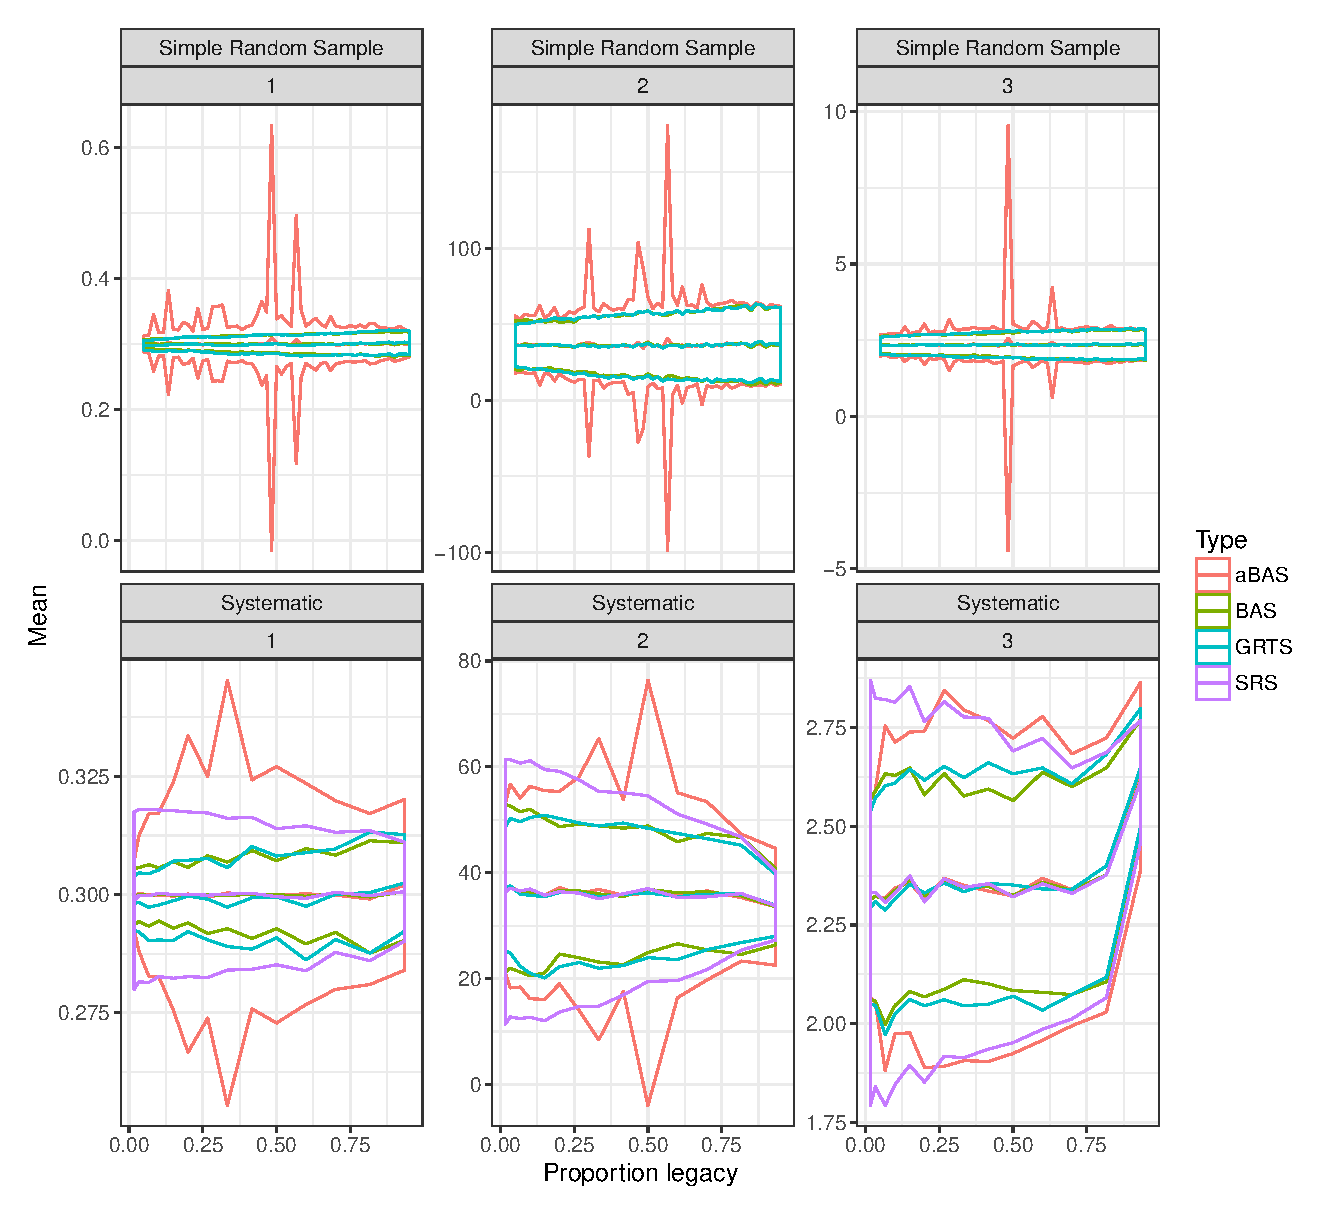
\includegraphics[scale = 0.5]{Estimation.eps}
	\caption{Results from the simulation study testing the impact of adding new samples from altered balanced acceptance sampling (aBAS), balanced acceptance sampling (BAS), generalised random tessellation stratified (GRTS), and simple random sampling (SRS) to existing legacy monitoring locations. Three populations with varying spatial structure were tested. Population 1, a strong spatial trend. Population 2, a peak function. Population 3, a cyclical (bird) function.}
	\label{estimation}
\end{figure}

\newpage


\begin{figure}[H]
	\centering
	\subfloat[]{\includegraphics[width=0.6\textwidth]{SIMS.eps}\label{NI1}}
	\hfill
	\subfloat[]{\includegraphics[width=0.6\textwidth]{Tier2EMUMS.eps}\label{NI2}}
	\caption{South Island of New Zealand (a) shows the first 5000 points of the master sample overlayed on red ecosystem management units (EMUs). (b) shows a sample size of 500 of master sample points from (a) that fall within the EMUs in red. Abel Tasman National Park receives seven samples which are included as the first seven in Figure \ref{Tasman}}
	\label{EMU}
\end{figure}

\newpage

\begin{figure}[H]
	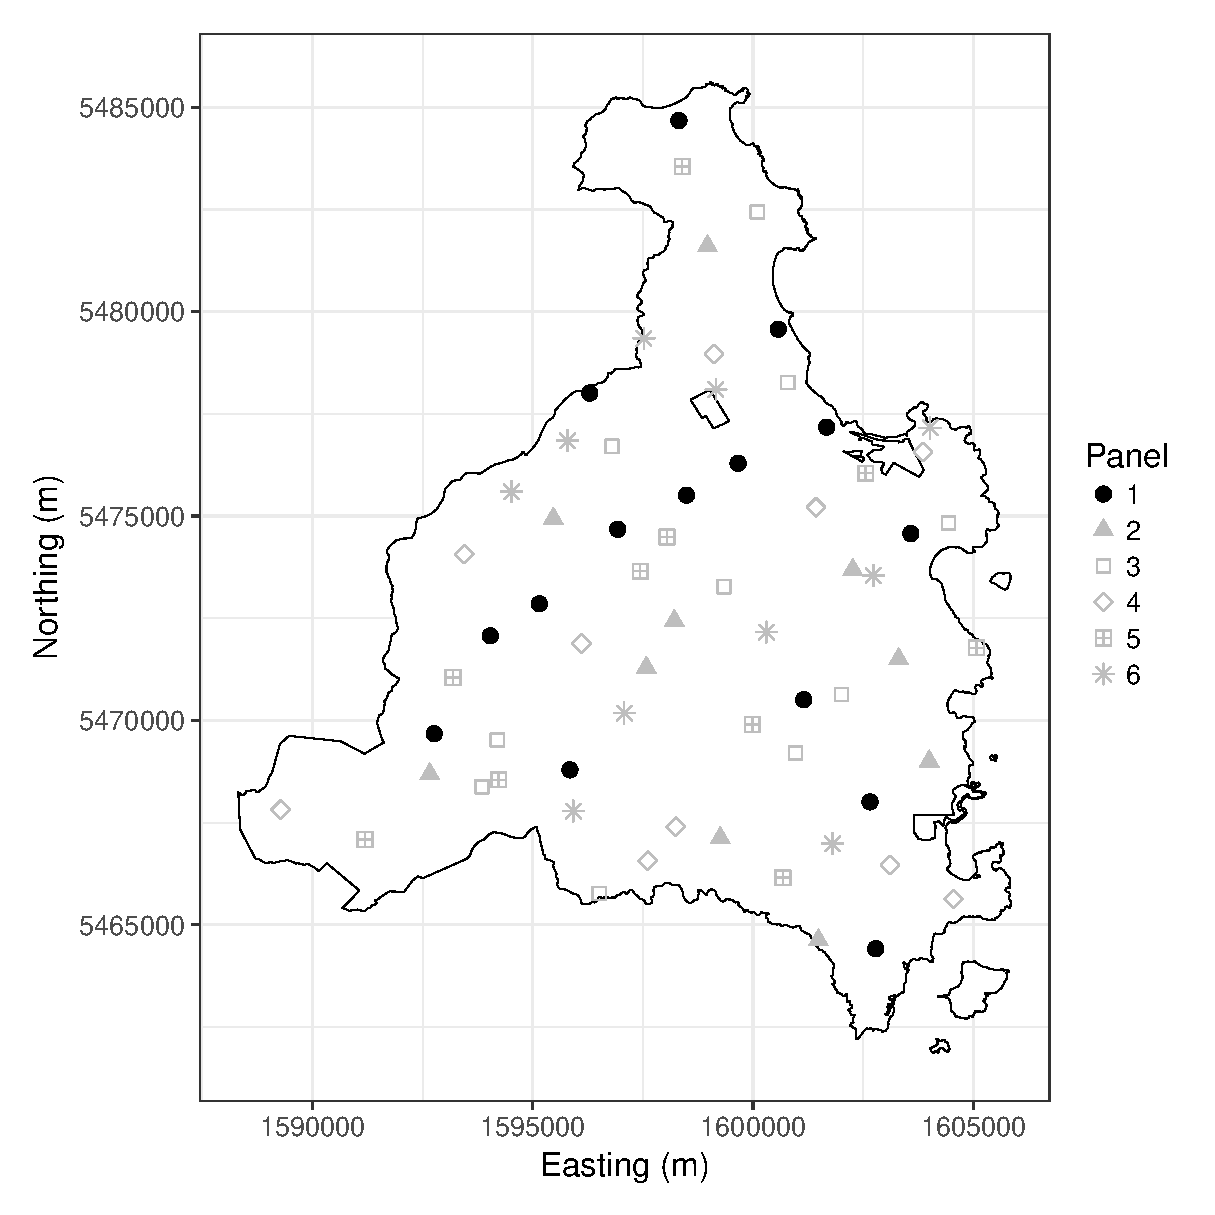
\includegraphics[width = \textwidth]{Tasman.eps}
	\caption{An example of bird monitoring in Abel Tasman National Park New Zealand. Panel 1 is measured annually while the other panels are on a 5-year rotation described as $[1-0,(1-4)^5]$. The first year, panels 1 and 2 would be sampled. This design gives excellent spatial coverage over the park each year ($n = 25$) and over a 5-year period ($n=65$).}
	\label{Tasman}
\end{figure}


\end{document}

Old abstract:
Environmental monitoring for management organisations like the Department of Conservation is critical. Without good information about outcomes, poor management actions may persist much longer than they should or initial  intervention may occur too late. The Department currently conducts focused research at key natural heritage sites (Tier 3) as well as a long term national monitoring (Tier 1). The link between the two tiers of investigation to assess the impact of management across New Zealand (Tier 2) is yet to be implemented but faces unique challenges for working at many different spatial scales and coordinating with multiple agencies. The solution is to implement a master sample using Balanced Acceptance Sampling (BAS). To do this some practical aspects of the sample design are addressed such as stratification, unequal probability sampling, rotating panel designs and regional intensification. Incorporating information from Tier 1 monitoring directly is also discussed.

The impact of intensifying sampling on the systematic grid using BAS was investigated by simulation. One hundred and twenty-one points on $[0,80]^2$ were generated systematically using the package sp in the program R \citep{R, sp1, sp2}. Simple Random Sampling (SRS), GRTS \citep{spsurvey}, and BAS points were added until spatial variance became stable ($n$ = 350). Spatial balance was measured using the variance of the Voronoi polygons \citep{Robertson2013, StevensOlsen2004, Grafstrom2012} and was repeated 300 times. Balanced Acceptance sampling was the best of the three methods for maintaining spatial balance Figure \ref{balance}. An example of what the intensified grid looked like with the Voronoi polygons can be seen in Figure \ref{voronoi}.